\subsection{RQ6: Controversial Influence}
\label{sec:rq6}

\paragraph{How much and which.} 2,458 candidates (3.9\%) carry at least one of the seven controversial mechanisms, slightly fewer than Python's 4.7\% (Table~\ref{tab:rq6}). The ordering is Python's with one change: incivility leads (1.43\%), then procedural control (0.78\%) and backchannel references (0.73\%), but corporate interest (0.49\%) comes next and ahead of unilateral decisions (0.22\%), which in Python were twice as frequent as corporate stakes. Gatekeeping (0.17\%) and exit threats (0.13\%) are rarer than in Python by about half. The Bitcoin numbers are also the more conservative ones: four rounds of cue tightening removed the technical homonyms (unilateral close, fork off, offline signing, out-of-band fees, dumb clients) that Bitcoin's vocabulary shares with the cue lists, and each round lowered the controversial share (from 4.7\% on the first full run to 3.9\%). Concentration follows the same pattern as in Python. Among BIPs with at least 150 candidates the highest densities belong to the process BIP itself (BIP~2, 9.0\%---the 2024 dispute over the editorship) and to the proposals the community remembers as contested: the covenant proposal BIP~119 (7.3\%), the dynamic block-size proposal BIP~100 (6.5\%), the activation proposal BIP~8 (4.9\%), the payment protocol BIP~70 (4.7\%) and Taproot's BIP~341 (4.4\%), against 3.5\% on BIPs that became final. Superseded and still-active BIPs carry the most (7.4\% and 7.3\%), rejected ones 4.8\%. By phase, the controversial share is highest before a BIP is assigned (6.1\%) and in its first month (5.3\%), and lowest after the recorded decision (3.3\%).

\begin{table}[t]
\caption{RQ6: controversial mechanisms in the Bitcoin corpus (62,789 candidates): count, share of all candidates, and share within each governance period.}
\label{tab:rq6}
\footnotesize
\setlength{\tabcolsep}{3.5pt}
\begin{tabular}{lrrrrrr}
\toprule
Mechanism & $n$ & \% all & Andresen & War & vdL & Post-lead \\
\midrule
Incivility & 900 & 1.43 & 1.30 & 1.34 & 1.04 & 1.80 \\
Procedural control & 488 & 0.78 & 0.55 & 0.40 & 0.54 & 1.33 \\
Backchannel & 456 & 0.73 & 2.36 & 0.63 & 0.69 & 0.59 \\
Corporate interest & 308 & 0.49 & 1.24 & 0.46 & 0.54 & 0.38 \\
Unilateral & 141 & 0.22 & 0.12 & 0.21 & 0.26 & 0.23 \\
Gatekeeping & 108 & 0.17 & 0.14 & 0.31 & 0.13 & 0.07 \\
Exit threat & 81 & 0.13 & 0.12 & 0.12 & 0.05 & 0.19 \\
\midrule
Any controversial & 2,458 & 3.9 & 5.8 & 3.4 & 3.2 & 4.6 \\
\bottomrule
\end{tabular}
\end{table}

\paragraph{Who.} Table~\ref{tab:rq6roles} gives the share of each role's candidates that carries each mechanism. The maintainers and the BIP editors are the most uncivil roles (2.57\% and 2.35\% of their candidates, against 1.30\% for community members)---the office-holders are the ones who lose patience---and the editors also lead on unilateral sentences (0.65\%), which in their case are the administrative formulas of their job (``I hereby assign BIP 42''). The lead maintainer's two holders wrote no exit threat, no procedural-control sentence and almost no backchannel reference; their controversial signals are corporate (0.76\%: Andresen on the Bitcoin Foundation and on companies' stakes, van der Laan on who is paid to work on Core) and, rarely, gatekeeping (``I refuse to take part in that''). Corporate-interest references are highest among community members (0.56\%), who are the ones pointing at employers: ``the position of Blockstream employees is that hard forks must never happen'' (BIP~100, 2015). Backchannel references are spread across all roles at 0.6--1.1\%, and the earliest period has by far the most (2.36\%): in 2012--2014 the editors repeatedly complained that decisions were being taken on IRC (``this discussion took place on IRC, and I never saw any of it \ldots BIP 1 says drafts should be evaluated on the mailing list'').

\begin{table}[t]
\caption{RQ6: share of each role's candidates carrying each controversial mechanism (\%).}
\label{tab:rq6roles}
\footnotesize
\setlength{\tabcolsep}{3pt}
\begin{tabular}{lrrrrrrrr}
\toprule
Role & $n$ & Unil. & Corp. & Gate. & Exit & Inciv. & Back. & Proc. \\
\midrule
Community member & 36,137 & 0.23 & 0.56 & 0.22 & 0.13 & 1.30 & 0.78 & 0.83 \\
Core developer & 17,045 & 0.19 & 0.38 & 0.11 & 0.13 & 1.58 & 0.62 & 0.77 \\
Proposal author & 6,179 & 0.23 & 0.49 & 0.13 & 0.10 & 1.36 & 0.70 & 0.65 \\
BIP editor & 1,530 & 0.65 & 0.20 & 0.00 & 0.13 & 2.35 & 1.05 & 0.72 \\
Maintainer & 1,243 & 0.00 & 0.32 & 0.08 & 0.16 & 2.57 & 0.64 & 0.40 \\
Lead maintainer & 655 & 0.31 & 0.76 & 0.31 & 0.00 & 1.07 & 0.15 & 0.00 \\
\bottomrule
\end{tabular}
\end{table}

\paragraph{Across the periods.} The controversial share is highest in the Andresen years (5.8\%), falls through the block-size war (3.4\%) and the post-war van der Laan years (3.2\%), and rises again in the post-lead era (4.6\%). The composition changes with it. The early years are marked by backchannel and corporate references (2.36\% and 1.24\%---IRC decisions and the Bitcoin Foundation); the war by gatekeeping at its peak (0.31\%) and by the lowest procedural control (0.40\%): the war was fought on the merits and with refusals, not with process. The post-lead era has the highest incivility (1.80\%), the highest exit-threat share (0.19\%), procedural control more than tripled (1.33\%) and gatekeeping at its lowest (0.07\%). Without a lead maintainer to refuse, the community argues about the process---who assigns numbers, what belongs on the list, what is out of scope---and does so more rudely. The same movement from persons to process that the Python paper found after the Steering Council appears here after the lead maintainer's departure, without any council to absorb it.

\paragraph{Examples.} Table~\ref{tab:rq6examples} shows sentences the tool labelled with each mechanism. They include the editor's refusal to accept a BIP negotiated on IRC (2012), the lead maintainer's rebuke of an author who changed his own BIP's status (2014), the accusation that Blockstream employees oppose all hard forks (2015), the proposal author's offer to withdraw BIPs 120 and 121 (2018), the activation-debate charge that developers ``become dictators who can unilaterally decide the rules'' (2021), the editor's dismissal of ``Ordinals nonsense'' (2023), a maintainer's ``ridiculous that we should be bottlenecked on simply what number a proposal should have'' (2024) and the editors' account of communication with a colleague having ``broken down'' (2026). They also show the limits of the cues in this corpus: ``I hereby assign BIP 42'' is an editor doing his job, ``no way that the miners are going to'' is a prediction rather than a refusal, and a BIP that says its reserved bits ``MUST NOT be used without community consensus'' is quoting a rule, not evading one.

\begin{table*}[t]
\caption{Sample sentences labelled with the controversial mechanisms (Bitcoin corpus; multi-label). Message text lightly trimmed.}
\label{tab:rq6examples}
\small
\begin{tabular}{p{0.135\textwidth}p{0.175\textwidth}p{0.63\textwidth}}
\toprule
Mechanism & BIP, author (role) & Sentence \\
\midrule
Unilateral & 42, Maxwell (BIP editor) & But owing to a rather large bribe (or at least not less large than any other offered by competing parties) I hereby assign BIP 42 for this proposal. \\
Unilateral & 8, Tim\'on (core dev.) & Most devs perceive that not giving miners veto power over proposals somehow means that then developers become dictators who can unilaterally decide the rules. \\
Unilateral & 101, Bishop (community) & Nothing about this should be an ``emergency'', we have all the time in the world to prepare a safe and responsible way to upgrade the network without unilaterally declaring obsolescence. \\
Unilateral & 360, Beast (author) & As such, I've decided to deprecate SQIsign from the BIP. \\
Corporate interest & 100, Hearn (core dev.) & No surprise, the position of Blockstream employees is that hard forks must never happen and that everyone's ordinary transactions should go via some new network that doesn't yet exist. \\
Corporate interest & 101, Hearn (core dev.) & I agree with Gavin---whilst it's great that a Blockstream employee has finally made a realistic proposal (i.e.\ not ``let's all use Lightning'')---this BIP is virtually the same as keeping the 1mb cap. \\
Gatekeeping & 66, van der Laan (lead maint.) & I refuse to take part in that. \\
Gatekeeping & 151, Voskuil (community) & Anonymous node identity is pointless, and is why I object to BIP151. \\
Gatekeeping & 101, Todd (core dev.) & No, I said there was no chance it'd be accepted ``due to a number of BIP-level issues in addition to debate about the patch itself''. \\
Exit threat & 120/121, Rosenbaum (author) & If there is no good solution to the soft-fork issue, I suggest that I withdraw BIP120 and BIP121. \\
Exit threat & 101, Garzik (core dev.) & Observation: Contentious hard fork is an Economic Change Event. \\
Incivility & 15, Andresen (lead maint.) & First: everybody please try to focus on the issues/ideas, and try to avoid this becoming a flame war. \\
Incivility & 8, Tim\'on (core dev.) & The only reason you don't like bip8 is because you're ignorant about it and you haven't reviewed it enough. join bip8, join us. do it for freedom. \\
Incivility & 69, Dashjr (BIP editor) & There are several PRs far more important than Ordinals nonsense that need to be triaged and probably merged. \\
Incivility & 2, Chow (maintainer) & It's ridiculous that we should be bottlenecked on simply what number a proposal should have. \\
Incivility & 65, Todd (author) & Unless you have an actual technical justification, arguments such as the above are highly dishonest and need to be removed from your BIP. \\
Backchannel & 22, Taaki (BIP editor) & However this discussion took place on IRC, and I never saw any of it to ascertain what happened (BIP 1 says drafts should be evaluated on the mailing list). \\
Backchannel & 1, van der Laan (lead maint.) & Changing your BIP status without community consensus is also not OK. \\
Backchannel & 102, Todd (core dev.) & Ironically that makes it harder to get a BIP \# if you know what you're doing, because Gregory Maxwell will argue against you in private and delay actually allocating one if he knows you should know better. \\
Backchannel & 110, Erhardt (BIP editor) & Communication between Luke and other BIP Editors had already broken down last year, following a discussion about his attempt to side-step the process by prematurely assigning a BIP number out of band. \\
Procedural control & 16, Taaki (BIP editor) & My feeling is that a BIP needs to go through the proper formalised motions in public before becoming accepted. \\
Procedural control & 44, Dashjr (core dev.) & Things which only improve altcoins, while a perfectly fine thing to standardise, are outside the scope of what belongs in a BIP. \\
Procedural control & 109, Corallo (core dev.) & I highly recommend you read the excellent thread on soft fork risks and respond there instead of getting off topic for this thread. \\
Procedural control & 3, Erhardt (author) & Since BIP 2 doesn't specify a procedure for activating Process BIPs, I suggest that people who wish to state their support leave an ACK on \#1820 or reply in this thread. \\
\bottomrule
\end{tabular}
\end{table*}

\subsection{Landmark Influence Acts Extracted from the Corpus}
\label{sec:landmarks}

Figure~\ref{fig:timeline} placed the events the community remembers on a timeline above the tool's measure of contestation. Figure~\ref{fig:timeline2} lets the tool nominate the landmarks. The rule differs from the Python study's, and the difference is itself a result: in Python the year's landmark was the highest-scoring decision-closing sentence by a decision-maker, and every year had one. In Bitcoin the lead maintainers, maintainers and editors produce almost no decision-closing sentences---their controversial signals are complaints about IRC, refusals to take part and administrative formulas---so the landmark act of each year is the highest-scoring sentence by \emph{any} participant that carries a controversial mechanism, chosen from the top seven to exclude quotations of BIP text and the technical homonyms the corpus still contains. Table~\ref{tab:landmarks} lists them; below the axis the figure stacks each year's candidates by the role of the writer.

Read in order, the acts tell a different story from Python's. There is no arc from pronouncement to delegation to council. There is an early period in which the editors fight to bring decisions from IRC onto the list and the lead maintainer polices status changes (2012--2014); a war in which the acts are refusals and accusations about who pays whom (2015--2017); a quiet period in which the acts are authors withdrawing and developers ruling things out of scope (2018--2020); and a post-lead period in which the acts are about the process itself---the activation debate's ``developers become dictators'' (2021), the editorship (2024, 2026), the process BIP's own activation (2025)---and about the tone of the list. The role bars show the lead maintainer's share vanishing after 2015, the editors' share spiking in the two editorship years (2012 and 2026), and core developers' share climbing from a fifth to a third and, in 2024, above half.

\begin{figure*}[t]
\centering
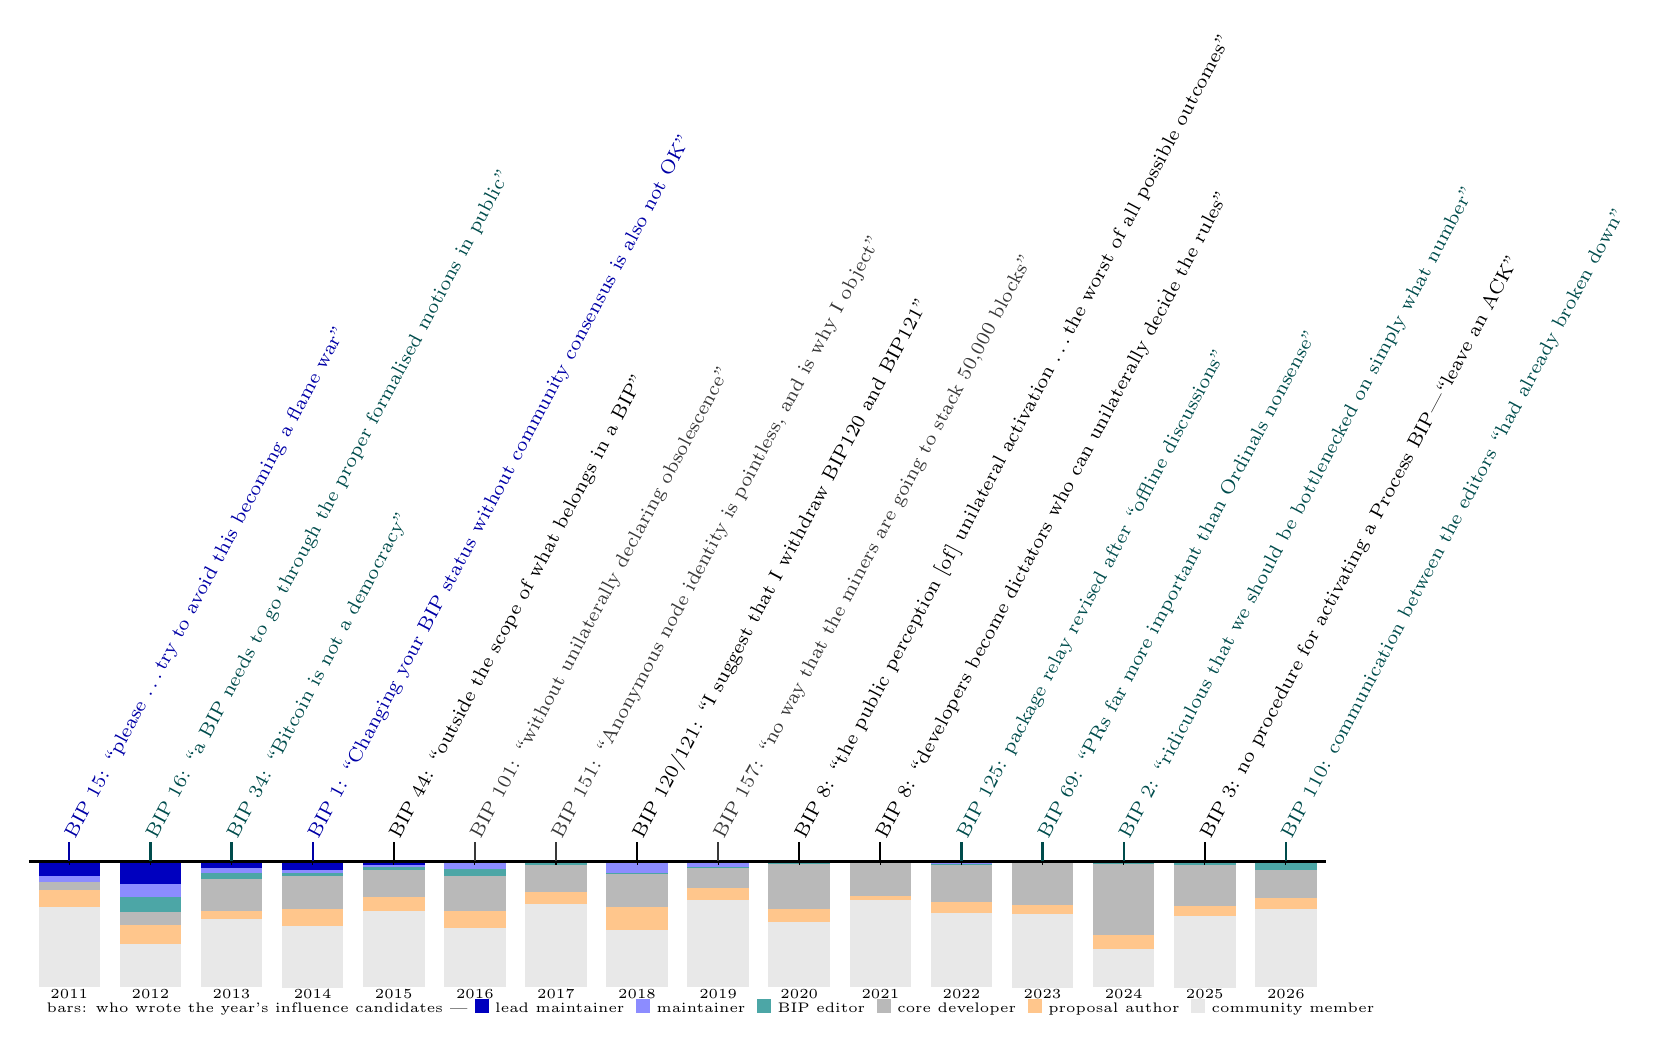
\begin{tikzpicture}[x=1.03cm, y=1cm, font=\scriptsize]
  % stacked role shares per year: lead maintainer, maintainer, BIP editor, core developer, proposal author, community
  \foreach \yr/\a/\b/\c/\d/\e/\f in {
    2011/11.7/4.4/0.0/6.3/13.6/64.0, 2012/17.8/10.8/11.8/9.7/15.1/34.8, 2013/5.4/3.7/4.6/25.3/6.7/54.3,
    2014/6.6/2.5/2.2/26.1/14.1/48.7, 2015/2.7/1.8/2.3/21.2/11.5/60.5, 2016/0.0/6.1/5.1/28.4/13.5/46.9,
    2017/0.0/0.8/2.2/21.3/9.4/66.3, 2018/0.0/9.5/0.5/25.9/18.5/45.6, 2019/0.0/4.7/0.5/15.9/9.2/69.7,
    2020/0.0/0.1/1.6/35.9/10.6/51.8, 2021/0.0/0.0/1.4/26.1/3.5/69.0, 2022/0.0/2.0/1.0/29.5/8.2/59.3,
    2023/0.0/0.8/0.4/33.1/7.8/58.0, 2024/0.0/0.7/1.7/56.2/10.8/30.5, 2025/0.0/0.2/2.5/32.3/8.0/57.1,
    2026/0.0/0.0/6.9/22.0/8.7/62.4} {
    \pgfmathsetmacro{\xl}{\yr-2011+0.12}
    \pgfmathsetmacro{\xr}{\yr-2011+0.88}
    \pgfmathsetmacro{\ya}{-\a*0.016}
    \pgfmathsetmacro{\yb}{\ya-\b*0.016}
    \pgfmathsetmacro{\yc}{\yb-\c*0.016}
    \pgfmathsetmacro{\yd}{\yc-\d*0.016}
    \pgfmathsetmacro{\ye}{\yd-\e*0.016}
    \pgfmathsetmacro{\yf}{\ye-\f*0.016}
    \fill[blue!75!black] (\xl,0) rectangle (\xr,\ya);
    \fill[blue!45] (\xl,\ya) rectangle (\xr,\yb);
    \fill[teal!70] (\xl,\yb) rectangle (\xr,\yc);
    \fill[gray!55] (\xl,\yc) rectangle (\xr,\yd);
    \fill[orange!45] (\xl,\yd) rectangle (\xr,\ye);
    \fill[gray!18] (\xl,\ye) rectangle (\xr,\yf);
  }
  \node[anchor=west, font=\tiny, align=left] at (0.1,-1.85) {bars: who wrote the year's influence candidates ---
    \textcolor{blue!75!black}{\rule{5pt}{5pt}} lead maintainer\;
    \textcolor{blue!45}{\rule{5pt}{5pt}} maintainer\;
    \textcolor{teal!70}{\rule{5pt}{5pt}} BIP editor\;
    \textcolor{gray!55}{\rule{5pt}{5pt}} core developer\;
    \textcolor{orange!45}{\rule{5pt}{5pt}} proposal author\;
    \textcolor{gray!18}{\rule{5pt}{5pt}} community member};
  \draw[thick] (0,0) -- (16,0);
  \foreach \yr in {2011,2012,...,2026} {
    \draw (\yr-2011+0.5,0.05) -- (\yr-2011+0.5,-0.05);
    \node[font=\tiny] at (\yr-2011+0.5,-1.68) {\yr};
  }
  \tikzset{lead/.style={blue!65!black}, ed/.style={teal!60!black}, dev/.style={black}, com/.style={gray!45!black}}
  \foreach \yr/\c/\t in {
    2011/lead/{BIP 15: ``please \ldots try to avoid this becoming a flame war''},
    2012/ed/{BIP 16: ``a BIP needs to go through the proper formalised motions in public''},
    2013/ed/{BIP 34: ``Bitcoin is not a democracy''},
    2014/lead/{BIP 1: ``Changing your BIP status without community consensus is also not OK''},
    2015/dev/{BIP 44: ``outside the scope of what belongs in a BIP''},
    2016/com/{BIP 101: ``without unilaterally declaring obsolescence''},
    2017/com/{BIP 151: ``Anonymous node identity is pointless, and is why I object''},
    2018/dev/{BIP 120/121: ``I suggest that I withdraw BIP120 and BIP121''},
    2019/com/{BIP 157: ``no way that the miners are going to stack 50,000 blocks''},
    2020/dev/{BIP 8: ``the public perception [of] unilateral activation \ldots the worst of all possible outcomes''},
    2021/dev/{BIP 8: ``developers become dictators who can unilaterally decide the rules''},
    2022/ed/{BIP 125: package relay revised after ``offline discussions''},
    2023/ed/{BIP 69: ``PRs far more important than Ordinals nonsense''},
    2024/ed/{BIP 2: ``ridiculous that we should be bottlenecked on simply what number''},
    2025/dev/{BIP 3: no procedure for activating a Process BIP---``leave an ACK''},
    2026/ed/{BIP 110: communication between the editors ``had already broken down''}} {
    \draw[\c, thick] (\yr-2011+0.5,0) -- (\yr-2011+0.5,0.25);
    \node[\c, rotate=62, anchor=west, inner sep=1pt] at (\yr-2011+0.5,0.27) {\t};
  }
\end{tikzpicture}
\caption{Landmark influence acts nominated by Influence Miner for Bitcoin, 2011--2026: for each year, the highest-scoring sentence carrying a controversial mechanism, coloured by the writer's role (dark blue: lead maintainer; teal: maintainer or BIP editor; black: core developer or proposal author; grey: community member); full sentences in Table~\ref{tab:landmarks}. Below the axis, the share of each year's influence candidates written by each role.}
\label{fig:timeline2}
\Description{A horizontal timeline from 2011 to 2026 with one short quoted sentence per year rising from the axis at an angle, and stacked bars below the axis showing the share of influence candidates written by each role per year; the lead maintainer's share disappears after 2015 and core developers' share grows.}
\end{figure*}

\begin{table*}[t]
\caption{The landmark influence acts of Figure~\ref{fig:timeline2}: for each year, the highest-scoring sentence carrying a controversial mechanism (score in brackets; mechanisms as labelled by the tool).}
\label{tab:landmarks}
\footnotesize
\begin{tabular}{p{0.03\textwidth}p{0.05\textwidth}p{0.15\textwidth}p{0.11\textwidth}p{0.58\textwidth}}
\toprule
Year & BIP & Author (role) & Mechanisms & Sentence \\
\midrule
2011 & 15 & Andresen (lead maint.) & tactical, incivility & First: everybody please try to focus on the issues/ideas, and try to avoid this becoming a flame war. [2.2] \\
2012 & 16 & Taaki (BIP editor) & procedural & My feeling is that a BIP needs to go through the proper formalised motions in public before becoming accepted. [3.3] \\
2013 & 34 & Maxwell (BIP editor) & unilateral & Bitcoin is not a democracy---it quite intentionally uses the consensus mechanism only for the one thing that nodes can not autonomously and interdependently validate (the ordering of transactions). [1.9] \\
2014 & 1 & van der Laan (lead maint.) & coalition, backchannel & Changing your BIP status without community consensus is also not OK. [3.0] \\
2015 & 44 & Dashjr (core dev.) & standards, procedural & Things which only improve altcoins, while a perfectly fine thing to standardise, are outside the scope of what belongs in a BIP. [3.4] \\
2016 & 101 & Bishop (community) & ecosystem, unilateral & Nothing about this should be an ``emergency'', we have all the time in the world to prepare a safe and responsible way to upgrade the network without unilaterally declaring obsolescence. [2.9] \\
2017 & 151 & Voskuil (community) & strategic, gatekeeping & Anonymous node identity is pointless, and is why I object to BIP151. [3.0] \\
2018 & 120 & Rosenbaum (author) & exit threat & If there is no good solution to the soft-fork issue, I suggest that I withdraw BIP120 and BIP121. [4.0] \\
2019 & 157 & Moral Agent (community) & ecosystem, economic, gatekeeping & There is no way that the miners are going to stack 50,000 blocks on top of an invalid block without the economic majority abandoning the invalid chain. [2.3] \\
2020 & 8 & Corallo (core dev.) & operational, unilateral & To not make every attempt to distance the activation method from the public perception unilateral activation strikes me as the worst of all possible outcomes for Bitcoin's longevity. [2.5] \\
2021 & 8 & Tim\'on (core dev.) & authority, ecosystem, unilateral & Most devs perceive that not giving miners veto power over proposals somehow means that then developers become dictators who can unilaterally decide the rules. [3.1] \\
2022 & 125 & Zhao (maintainer) & operational, ecosystem, backchannel & I've made some significant changes to my package relay proposal based on observations while implementing, feedback on this thread, and offline discussions. [3.0] \\
2023 & 69 & Dashjr (BIP editor) & incivility & There are several PRs far more important than Ordinals nonsense that need to be triaged and probably merged. [2.5] \\
2024 & 2 & Chow (maintainer) & incivility & It's ridiculous that we should be bottlenecked on simply what number a proposal should have. [3.2] \\
2025 & 3 & Erhardt (author) & procedural & Since BIP 2 doesn't specify a procedure for activating Process BIPs, I suggest that people who wish to state their support leave an ACK on \#1820 or reply in this thread. [3.9] \\
2026 & 110 & Erhardt (BIP editor) & authority, ecosystem, backchannel & Communication between Luke and other BIP Editors had already broken down last year, following a discussion about his attempt to side-step the process by prematurely assigning a BIP number out of band. [3.1] \\
\bottomrule
\end{tabular}
\end{table*}

